\section{Preparação e distribuição de ar comprimido}

\begin{frame}{Introdução}
	\begin{block}{}
		O ar comprimido deve ser \textbf{preparado antes de ser utilizado pelo sistema pneumático}, já que vem da atmosfera \textbf{úmido} e \textbf{misturado a outras substâncias ou partículas} que podem ser prejudiciais ao sistema de trabalho, e por isso deve ser \textbf{filtrado} e \textbf{secado}.
	\end{block}
\end{frame}


\begin{frame}{Umidade}
\begin{block}{Introdução}
	Quando o ar é \textbf{aquecido} no processo de compressão, sua capacidade de reter água é \textbf{amplificada}, podendo causar problemas conforme percorre as linhas de ar.
	
	Os problemas da \textbf{condensação de água} na linha incluem:
	\begin{itemize}
		\item Oxidação da tubulação e dos componentes pneumáticos.
		\item Destruição da película lubrificante existente entre as duas
		superfícies que estão em contato, acarretando desgaste
		prematuro e reduzindo a vida útil das peças, válvulas,
		cilindros, etc.
		\item Arrastamento de partículas sólidas que prejudicarão o funcionamento dos componentes pneumáticos.
		\item Aumento do índice de manutenção.
		\item Impossibilita a aplicação em equipamentos de pulverização.
		\item Provoca golpes de ariete nas superfícies adjacentes, etc.
	\end{itemize}
\end{block}
\end{frame}


\begin{frame}{Umidade}
	\begin{block}{Resfriador posterior}
		O \textbf{resfriador posterior} permite que esses problemas sejam resolvidos resfriando o ar após sua saída do compressor.
	\end{block}

	\centering
	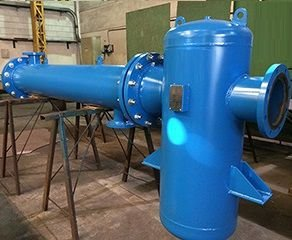
\includegraphics[width=0.6\linewidth]{Figuras/Ch13/fig1}
\end{frame}


\begin{frame}{Reservatório}
	\begin{block}{}
		O reservatório deve:
		\begin{itemize}
			\item Armazenar o ar comprimido.
			\item Resfriar o ar auxiliando a eliminação do condensado.
			\item Compensar as flutuações de pressão em todo o sistema de distribuição.
			\item Estabilizar o fluxo de ar.
			\item Entre outras funções...
		\end{itemize}
	\end{block}
	
	\centering
	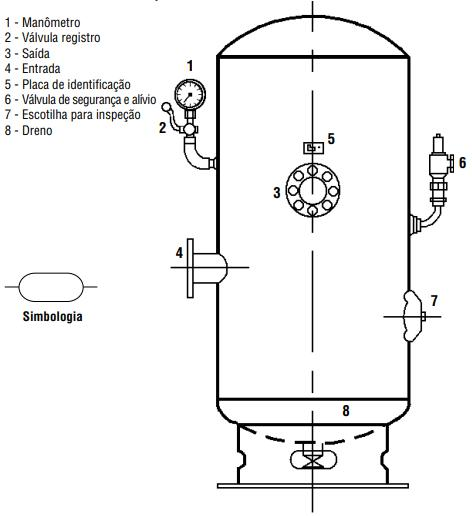
\includegraphics[height=0.5\textheight]{Figuras/Ch13/fig2}
\end{frame}


\begin{frame}{Filtro}
	\begin{block}{}
		Também é importante a instalação de filtros no sistema de preparação do ar comprimido.
		
		Estes podem ser:
		\begin{itemize}
			\item \textbf{Pré-filtro}
			
			Instalado antes do secador para separar contaminantes sólidos e líquidos.
			\item \textbf{Pós-filtro}
			
			Instalado após o secador para retirar a umidade residual, além de sólidos não retidos no pré-filtro (dupla filtragem).
		\end{itemize}
	\end{block}
\end{frame}


\begin{frame}{Filtro}
	\centering
	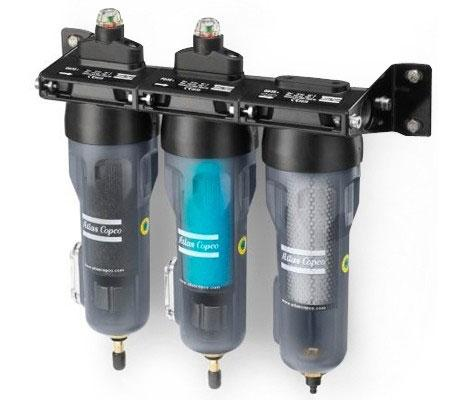
\includegraphics[height=0.8\textheight]{Figuras/Ch13/fig3}
	
	Filtro coalescente industrial
\end{frame}


\begin{frame}{Secadores de ar}
	\begin{block}{}
		A presença de umidade no ar comprimido é sempre prejudicial
		para as automatizações pneumáticas, pois causa sérias
		consequências, portanto é necessário \textbf{eliminar} ou \textbf{reduzir ao máximo} esta umidade.
		
		Isso pode ser feito com um \textbf{secador de ar.}
	\end{block}
\end{frame}


\begin{frame}{Secadores de ar}
	\begin{block}{Secagem por refrigeração}
		Consiste em submeter o ar a uma temperatura
		suficientemente baixa, a fim de que a quantidade de água existente seja retirada em grande parte já que a capacidade do ar de reter umidade é diretamente proporcional à temperatura.
	\end{block}

	\begin{minipage}{0.45\linewidth}
		\centering
		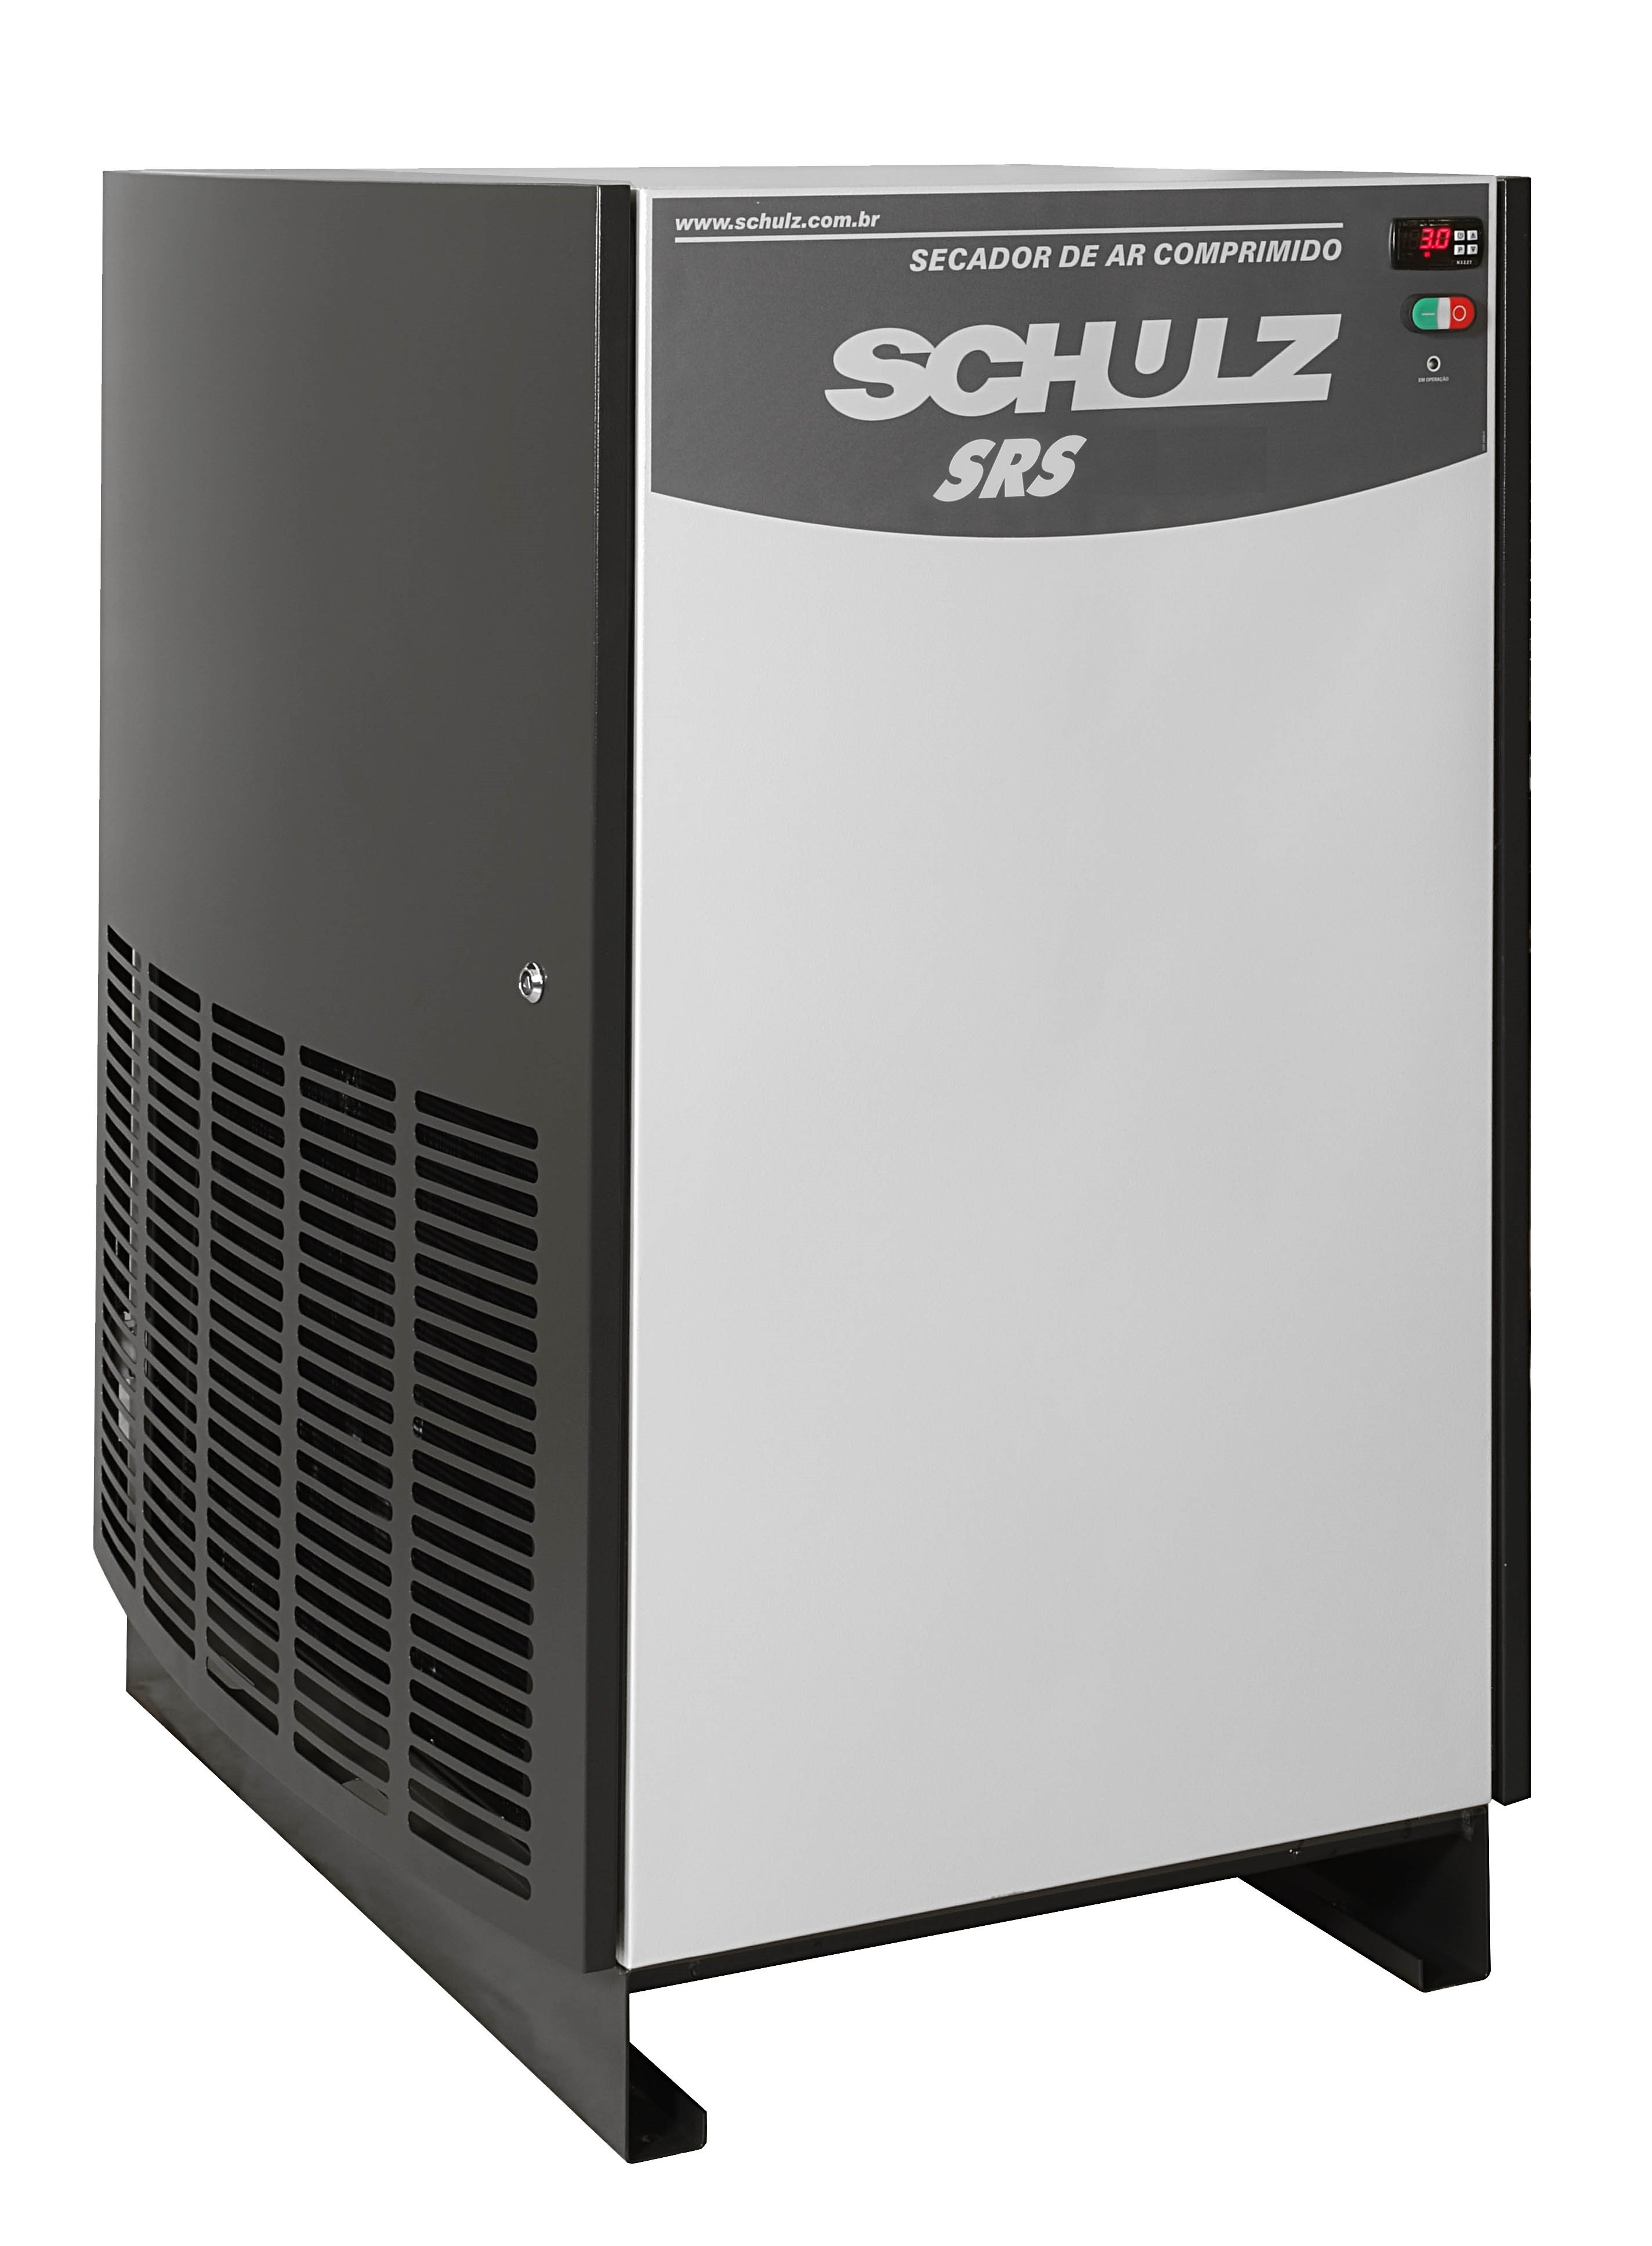
\includegraphics[width=0.7\linewidth]{Figuras/Ch13/fig4}
	\end{minipage}
	\hfill
	\begin{minipage}{0.45\linewidth}
		\centering
		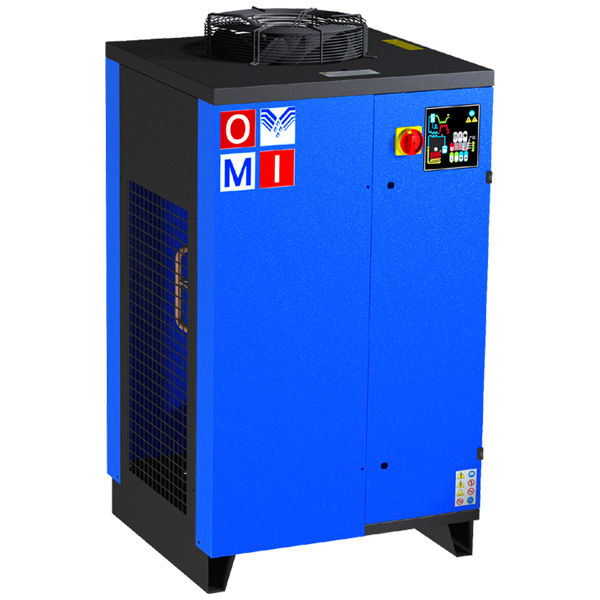
\includegraphics[width=0.9\linewidth]{Figuras/Ch13/fig5}
	\end{minipage}
\end{frame}


\begin{frame}{Secadores de ar}
	\centering
	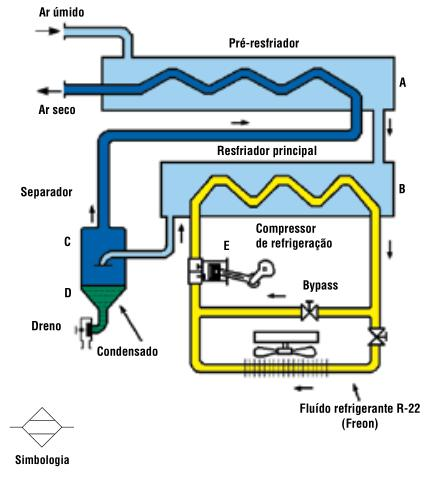
\includegraphics[height=0.8\textheight]{Figuras/Ch13/fig6}
	
	Diagrama de funcionamento do secador por refrigeração
\end{frame}


\begin{frame}{Secadores de ar}
	\begin{block}{Secagem por absorção}
		\begin{itemize}
			\item É o método que utiliza, em um circuito, uma substância sólida ou líquida, com capacidade de absorver outra substância líquida ou gasosa.
			
			\item A umidade retirada e a substância diluída são depositadas na parte inferior do invólucro, junto a um dreno, de onde são	eliminadas para a atmosfera.
			
			\item As principais substâncias utilizadas são:
			\begin{itemize}
				\item Cloreto de Cálcio.
				\item Cloreto de Lítio.
				\item Dry-o-Lite.
			\end{itemize}
			
			\item Com a consequente diluição das substâncias, é necessária uma reposição regular, caso contrário o processo torna-se deficiente.
			
			\item Este processo é também chamado de Processo Químico de Secagem.
		\end{itemize}
	\end{block}
\end{frame}


\begin{frame}{Secadores de ar}
	\centering
	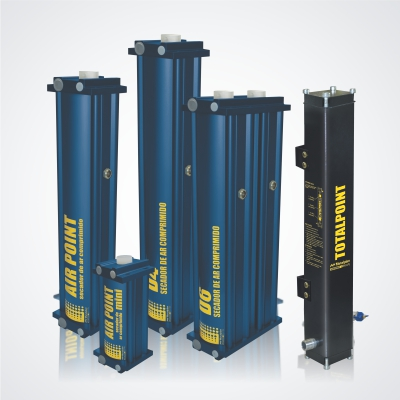
\includegraphics[height=0.8\textheight]{Figuras/Ch13/fig7}
	
	Secador por absorção
\end{frame}


\begin{frame}{Secadores de ar}
	\begin{block}{Secagem por adsorção}
		\begin{itemize}
			\item É a fixação das moléculas de um adsorvato na superfície de um adsorvente geralmente poroso e granulado, ou seja, é o processo de depositar moléculas de uma substância (ex. água) na superfície de outra substância, geralmente sólida (ex. SiO$_2$).
				
			\item Este método também é conhecido por Processo Físico de Secagem, porém seus detalhes são desconhecidos.
			
			\item O processo de adsorção é regenerativo; a substância adsorvente, após estar saturada de umidade, permite a liberação de água quando submetida a um aquecimento	regenerativo.
		\end{itemize}
	\end{block}
\end{frame}


\begin{frame}{Secadores de ar}
	\centering
	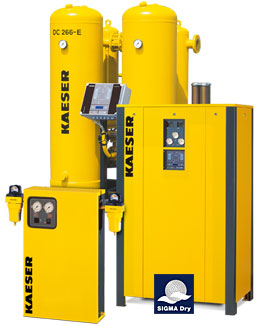
\includegraphics[height=0.8\textheight]{Figuras/Ch13/fig8}
	
	Secador por adsorção
\end{frame}


\begin{frame}{Produção, armazenamento e condicionamento do ar comprimido}
	\centering
	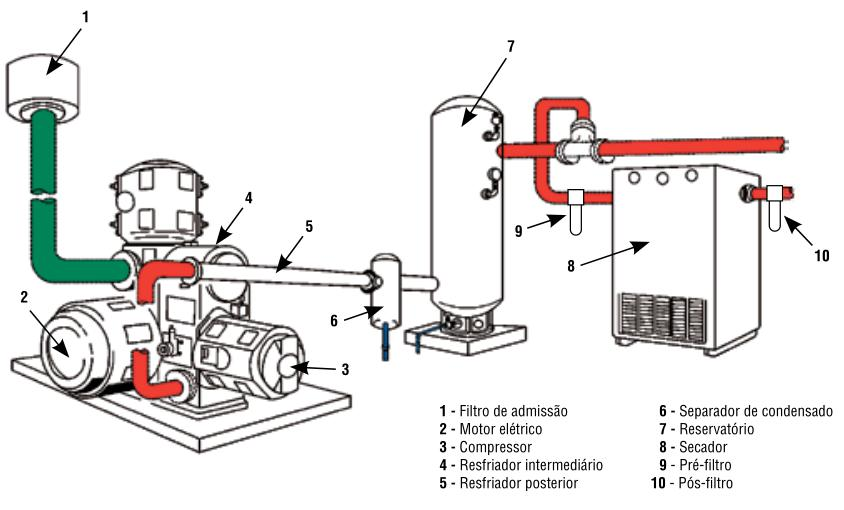
\includegraphics[width=1\linewidth]{Figuras/Ch13/fig9}
\end{frame}


\begin{frame}{Redes de distribuição}
	\begin{block}{}
		\begin{itemize}
			\item Como \textbf{não} é econômico usar \textbf{um compressor distinto para cada dispositivo pneumático} num sistema, a alternativa, então, é \textbf{distribuir o ar comprimido para vários dispositivos através de uma rede.}
			\item A \textit{rede de distribuição de ar comprimido }compreende \textbf{todas as tubulações} que saem do reservatório e que, unidas, \textbf{orientam o ar comprimido} até os pontos individuais de utilização.
			\item A rede possui duas funções básicas:
			\begin{enumerate}
				\item Comunicar a fonte produtora com os equipamentos
				consumidores.
				\item Funcionar como um reservatório para atender às exigências locais.
			\end{enumerate}
		\end{itemize}
	\end{block}
\end{frame}


\begin{frame}{Redes de distribuição}
	\begin{block}{}
		Um sistema de distribuição \textbf{perfeitamente executado} deve
		apresentar os seguintes requisitos:
		
		\begin{itemize}
			\item \textbf{Pequena queda de pressão entre o compressor e as partes de consumo}, a fim de manter a pressão dentro de limites toleráveis em conformidade com as exigências das aplicações.
			\item \textbf{Não apresentar escape de ar;} do contrário haveria perda de potência.
			\item Apresentar grande capacidade de realizar separação de condensado.
		\end{itemize}
	
		Esses itens devem ser considerados no \textbf{projeto} e \textbf{instalação} de \textbf{qualquer planta de distribuição} para o devido funcionamento do sistema pneumático e para que \textbf{não haja grande necessidade de manutenção.}
		
		\smallskip
		
		Para o cumprimento dos requisitos apresentados, há de se estudar algumas características das redes.
	\end{block}
\end{frame}


\begin{frame}{Redes de distribuição}
	\begin{block}{Layout}
		É a característica responsável por:
		\begin{itemize}
			\item Ramificações.
			\item Pontos de consumo.
			\item Pressão destes pontos.
			\item Posição de válvulas de fechamento.
			\item Moduladoras.
			\item Conexões.
			\item Curvaturas.
			\item Separadores de condensado.
			\item Etc.
		\end{itemize}
		Através do layout, pode-se então definir o \textbf{menor percurso
		da tubulação}, acarretando \textbf{menores perdas de carga} e
		proporcionando \textbf{economia}.
	\end{block}
\end{frame}


\begin{frame}{Redes de distribuição}
	\begin{block}{Formato}
			
			Em relação ao tipo de linha a ser executado, anel fechado (circuito fechado) ou circuito aberto, devem-se analisar as condições favoráveis e desfavoráveis de cada uma.
			
			Geralmente a rede de distribuição é em \textbf{circuito fechado}, em torno da área onde há necessidade do ar comprimido. Deste anel partem as ramificações para os diferentes pontos de consumo.
	\end{block}

	\centering
	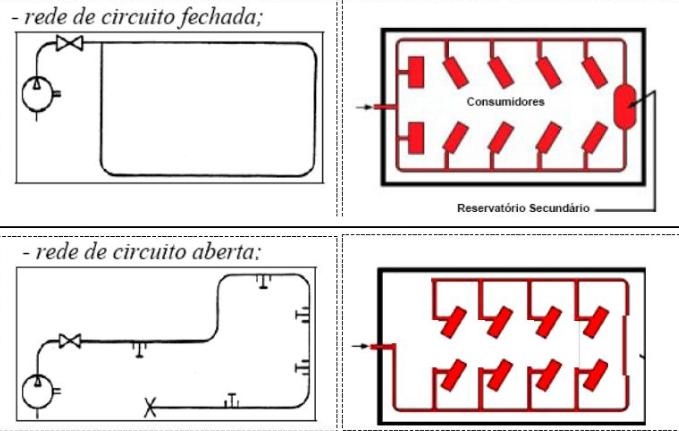
\includegraphics[width=0.5\linewidth]{Figuras/Ch13/fig10}
	
\end{frame}


\begin{frame}{Redes de distribuição}
	\begin{block}{Válvulas de fechamento na linha de distribuição}
			
			São de grande importância na rede de distribuição para permitir a divisão desta em \textbf{seções}, especialmente em casos de grandes redes, fazendo com que as seções tornem-se isoladas para \textbf{inspeção, modificações e manutenção}.
			
			Assim, evitamos que outras seções sejam simultaneamente atingidas, não havendo \textbf{paralisação do trabalho e da produção}.
	\end{block}
	\begin{block}{Ligações entre os tubos}
		\begin{itemize}
			\item Há várias possibilidades (rosca, solda, flange,
			acoplamento rápido, etc.).
			\item Cada uma tem seus prós e contras para determinado ambiente e diâmetro da tubulação.
		\end{itemize}
	\end{block}
\end{frame}


\begin{frame}{Redes de distribuição}
	\begin{block}{Curvatura}
		As curvas devem ser feitas no \textbf{maior raio possível}, para evitar \textbf{perdas excessivas por turbulência}. Evitar sempre a colocação de cotovelos \ang{90}. A \textbf{curva mínima} deve possuir na curvatura interior um raio mínimo de \textbf{duas vezes o diâmetro externo} do tubo.
	\end{block}

	\centering
	
\includegraphics[width=0.4\linewidth]{Figuras/Ch13/fig11}

\end{frame}


\begin{frame}{Redes de distribuição}
	\begin{block}{Inclinação}
	\begin{itemize}
		\item As tubulações devem possuir uma determinada \textbf{inclinação no sentido do fluxo}, pois se a temperatura da tubulação baixar, haverá, embora raramente, \textbf{precipitação de água}.
		\item A inclinação serve para favorecer o \textbf{recolhimento} desta \textbf{eventual condensação} e das \textbf{impurezas} devido à formação de óxido, levando-as para o ponto mais baixo, onde são \textbf{eliminadas} para a atmosfera, através do dreno.
		\item O valor desta inclinação é de \num{0.5} a 2\% em função do comprimento reto da tubulação onde for executada.
		\item Se a rede é relativamente extensa, recomenda-se observar a colocação de \textbf{mais de um dreno}, distanciados aproximadamente 20 a \SI{30}{\meter} um do outro.
	\end{itemize}
	\end{block}
\end{frame}


\begin{frame}{Redes de distribuição}
	\begin{block}{Drenagem de umidade}
		Com os cuidados vistos anteriormente para eliminação do condensado, resta uma umidade remanescente, a qual deve ser \textbf{removida} ou até mesmo \textbf{eliminada}, em caso de condensação da mesma.

		\begin{itemize}
			\item Para que a drenagem eventual seja feita, devem ser instalados \textbf{drenos} (purgadores), que podem ser manuais ou automáticos, \textbf{com preferência para o último tipo}. Os pontos de drenagem devem se situar em \textbf{todos os locais baixos} da tubulação: fim de linha, onde houver elevação de linha, etc.
			\item Nestes pontos, para auxiliar a eficiência da drenagem, podem ser construídos \textbf{bolsões}, que \textbf{retêm o condensado} e o encaminham para o purgador. Estes bolsões, construídos, \textbf{não} devem possuir diâmetros \textbf{menores} que o da tubulação. O ideal é que sejam do \textbf{mesmo tamanho}.
		\end{itemize}
	\end{block}

\end{frame}


\begin{frame}{}
	\centering
	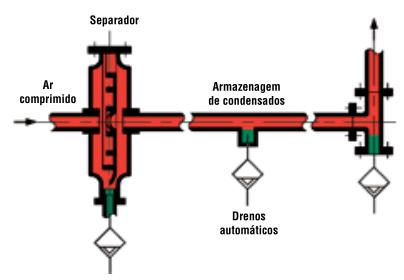
\includegraphics[width=0.9\linewidth]{Figuras/Ch13/fig12}
	
	Prevenção e drenagem para o condensado
\end{frame}


\begin{frame}{Redes de distribuição}
	\begin{block}{Tomadas de ar}
		\begin{itemize}
			\item Devem ser sempre feitas pela parte \textbf{superior} da tubulação principal, para evitar os \textbf{problemas de condensado} já expostos.
			\item Recomenda-se ainda que não se realize a \textbf{utilização direta} do ar no ponto terminal do tubo de tomada.
			\item No terminal, deve-se colocar uma pequena \textbf{válvula de drenagem} e a utilização deve ser feita \textbf{um pouco mais acima}, onde o ar, antes de ir para a máquina, passa através da \textbf{unidade de condicionamento}.
		\end{itemize}
	
	\end{block}

	\centering
	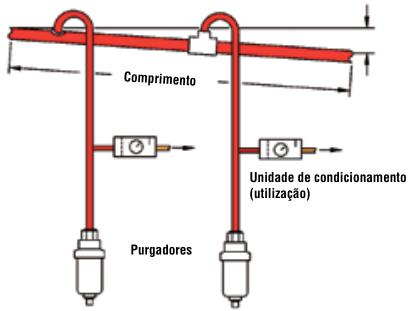
\includegraphics[width=0.4\linewidth]{Figuras/Ch13/fig13}

\end{frame}


\begin{frame}{Redes de distribuição}
	\begin{block}{Materiais da tubulação principal}
		Com relação aos materiais da tubulação, a preferência deve ser dada aos \textbf{resistentes à oxidação}, como aço galvanizado, aço inoxidável, alumínio, cobre e plástico de engenharia.
	\end{block}
\end{frame}


\begin{frame}{Redes de distribuição}
	\begin{block}{Tubulações secundárias}
		A seleção dos tubos que irão compor a instalação secundária e os materiais de que são confeccionados são fatores importantes, bem como o tipo de acessório ou conexão a ser utilizado.
		
		\begin{itemize}
			\item Devem-se ter materiais de \textbf{alta resistência}, durabilidade, etc.
			
			\item O processo de tubulação secundária sofreu uma evolução bastante rápida: o tubo de cobre, até bem pouco tempo, era um dos mais usados. Atualmente ele é utilizado em instalações mais específicas, montagens rígidas e locais em que a temperatura e a pressão são elevadas.
			
			\item Hoje são utilizados \textbf{tubos sintéticos}, os quais proporcionam boa resistência mecânica, apresentando uma elevada força de ruptura e grande flexibilidade. São usados tubos de polietileno, poliuretano e tubos nylon.
		\end{itemize}
	\end{block}
\end{frame}


\begin{frame}{Redes de distribuição}
	\begin{block}{Vazamentos}
		\begin{itemize}
			\item As quantidades de ar perdidas através de pequenos furos, acoplamentos com folgas, vedações defeituosas, etc., quando somadas, alcançam \textbf{elevados valores}.
			
			\item A importância econômica desta contínua perda de ar torna-se \textbf{mais evidente} quando comparada com o consumo de um equipamento e a potência necessária para realizar a compressão.
			
			\item É \textbf{impossível} eliminar por completo todos os vazamentos, porém estes devem ser \textbf{reduzidos ao máximo} com uma \textbf{manutenção preventiva} do sistema, de 3 a 5 vezes por ano, sendo verificados, por exemplo: substituição de juntas de vedação defeituosa, engates, mangueiras, tubos, válvulas, aperto das conexões, restauração das vedações nas uniões roscadas, eliminação dos ramais de distribuição fora de uso e outras que podem aparecer, dependendo da rede construída.
		\end{itemize}
	\end{block}
\end{frame}


\begin{frame}{Redes de distribuição}
	\begin{block}{Vazamentos}
		\begin{itemize}
			\item Desta forma, um vazamento na rede representa um consumo \textbf{consideravelmente maior} de energia, que pode ser verificado através da tabela abaixo.
		\end{itemize}
		
	\end{block}
	
	\centering
	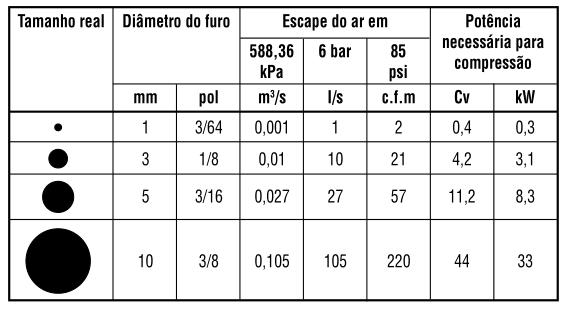
\includegraphics[width=0.8\linewidth]{Figuras/Ch13/fig15}
	
\end{frame}


\begin{frame}{Unidade de condicionamento}
	\begin{block}{Introdução}
		\begin{itemize}
			\item Após passar por todo o processo de produção, tratamento e distribuição, o ar comprimido deve sofrer um \textbf{último condicionamento}, antes de ser colocado para trabalhar, a fim de produzir melhores desempenhos.
		\end{itemize}
	\end{block}
	
%	\centering
%	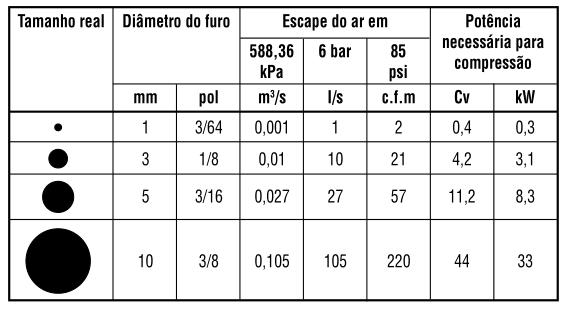
\includegraphics[width=0.8\linewidth]{Figuras/Ch13/fig15}
	
\end{frame}


\begin{frame}{Unidade de condicionamento}
	\begin{block}{Filtro de ar}
		\begin{itemize}
			\item Separa partículas normalmente abrasivas e auxilia na remoção da umidade remanescente pela ação centrífuga e por meio do elemento filtrante.
		\end{itemize}
	\end{block}

	\centering
	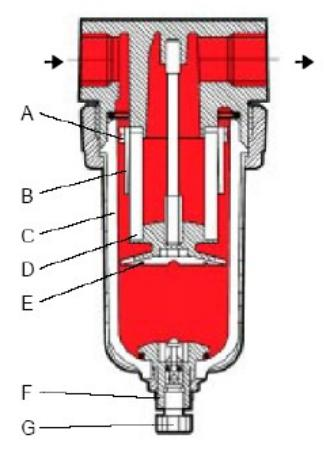
\includegraphics[height=0.6\textheight]{Figuras/Ch13/fig16}
	
\end{frame}


\begin{frame}{Unidade de condicionamento}
	\begin{block}{Reguladora de pressão}
		As reguladoras foram projetadas para proporcionar uma \textbf{resposta rápida} e uma \textbf{regulagem de pressão acurada} para o maior número de aplicações industriais. O uso do diafragma especialmente projetado resulta em um aumento significativo da vida útil da reguladora, proporcionando \textbf{baixos custos de manutenção}.
		
		\smallskip
		
		Características principais:
		\begin{itemize}
			\item Resposta rápida e regulagem precisa, devido a uma aspiração secundária e a válvula de assento incorporada.
			\item Grande capacidade de reversão de fluxo.
			\item Diafragma projetado para proporcionar um aumento da vida útil do produto.
			\item Dois orifícios destinados a manômetro, que podem ser usados como orifícios de saída.
			\item Fácil manutenção.
		\end{itemize}
	\end{block}
\end{frame}


\begin{frame}{Unidade de condicionamento}
	\centering
	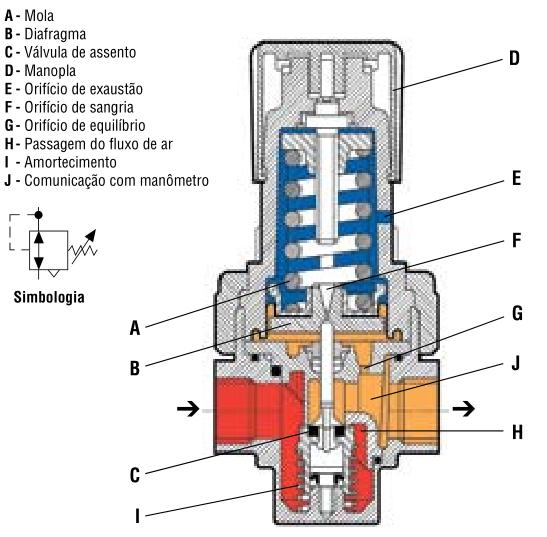
\includegraphics[height=0.8\textheight]{Figuras/Ch13/fig17}
	
	Reguladora de pressão em corte
\end{frame}


\begin{frame}{Unidade de condicionamento}
	\begin{block}{Lubrificador}
		O elemento lubrificante é necessário para garantir um \textbf{desgaste mínimo} dos elementos móveis através da \textbf{redução da força de atrito} e também para protegê-los contra \textbf{corrosão}.
	\end{block}

	\centering
	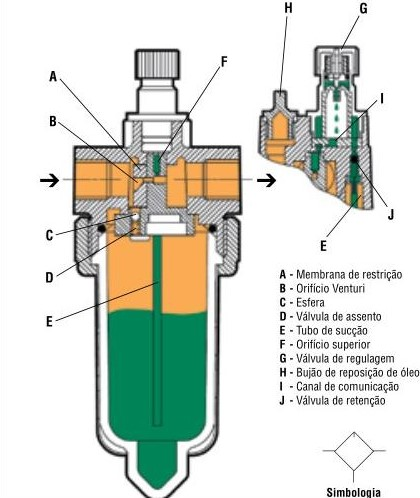
\includegraphics[height=0.6\textheight]{Figuras/Ch13/fig18}

\end{frame}


\frame{
	\frametitle{Exercícios}
	\begin{block}{}
		01. Na bancada de trabalho o ar comprimido não apresenta pressão suficiente para o serviço. Qual elemento pode ser o culpado?
		
		\vspace{0.5cm}
		
		02. O engenheiro responsável por um projeto pneumático recomendou a instalação de um novo sistema de filtragem após encontrar oxidação em diversos componentes de trabalho. Ele está correto em sua decisão? Justifique.
	\end{block}
}

\section*{Referências}
\frame{
	\frametitle{Referências e Exercícios Complementares}
	\begin{itemize}
		\item MELCONIAN, Sarkis. Sistemas Fluidomecânicos - Hidráulica e Pneumática, 1 ed. Érica, 2014.
	\end{itemize}
	%\centering{\alert{Página 546 - \textbf{Capítulo 6}}} \\
	%\centering{\alert{Lista de exercícios 01}}
}
